% \begin{figure*}[ht]
%     \centering
%     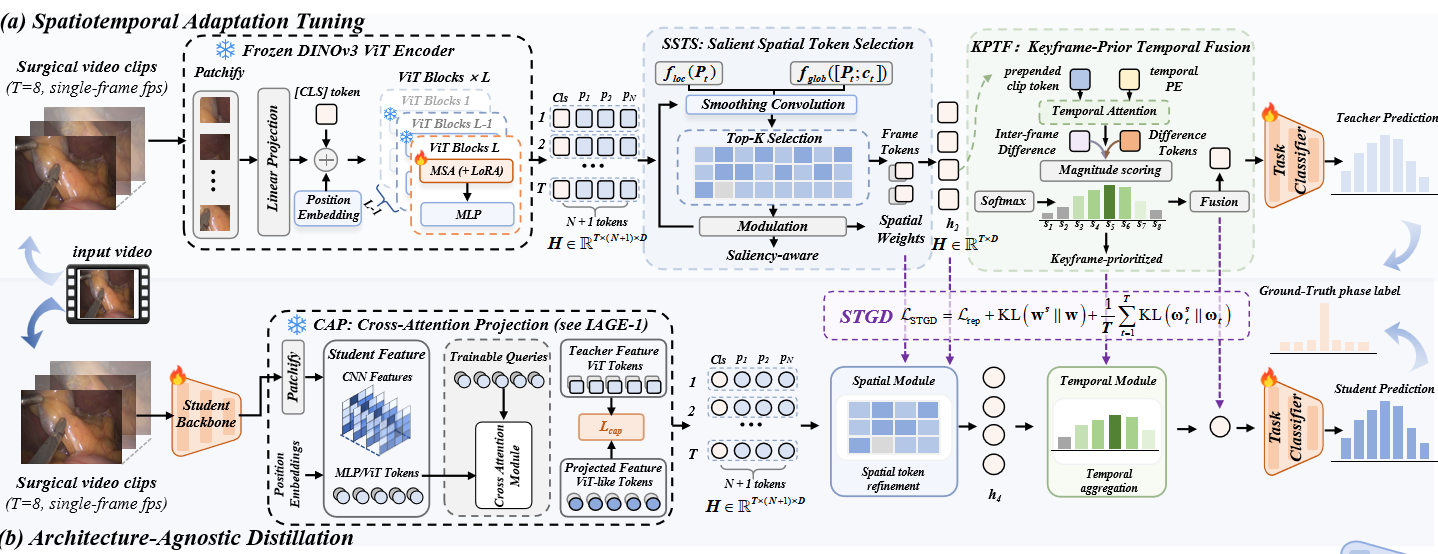
\includegraphics[width=\textwidth]{resources/method.png}
%     \caption{Visualization for our method.}
%     \label{fig:method}
% \end{figure*}


\section{Method}
\label{sec:method}

% Method overview / pipeline figure
\begin{figure*}[t]
    \centering
    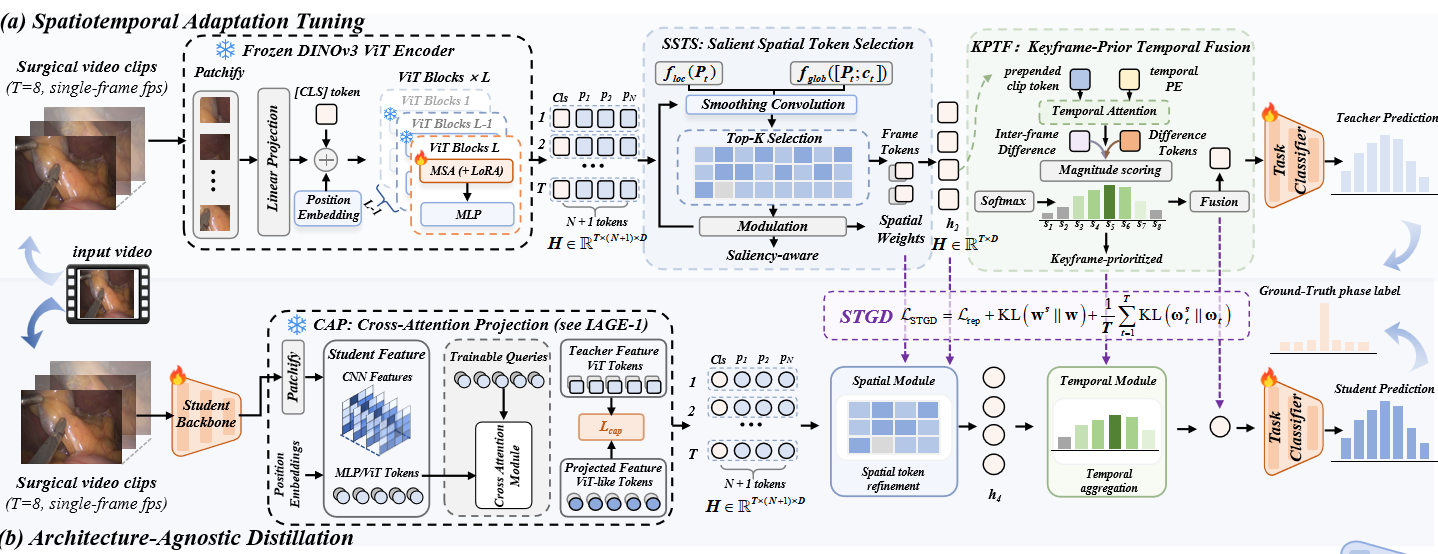
\includegraphics[width=\textwidth]{resources/method.png}
    \caption{Overview of the proposed framework. A frozen DINOv3 backbone is adapted to surgical video through a
    Salient Spatial Token Selection (SSTS) module and a Keyframe-Prior Temporal Fusion (KPTF)
    module, yielding SPR-Teacher. SPR-Lite further compresses the adapted model into lightweight backbones of
    arbitrary architectures via architecture-agnostic distillation.}
    \label{fig:method}
\end{figure*}



% ════════════════════════════════════════════════════════════════════
% TODO 图：整体 pipeline（视频适配 → 架构-无知蒸馏）
%   资源：figures/fig_pipeline.pdf（待制作）
% ════════════════════════════════════════════════════════════════════

\subsection{Overview}
\label{sec:method:overview}

% 写作要点（缩写 SSTS/KPTF/CAP/STGD 已在 intro 展开，本节不再重复给全称）：
% - 段 1：整体 roadmap——SPR-Teacher = DINOv3 + spatiotemporal 适配（SSTS 空间 + KPTF
%   时序），SPR-Lite = architecture-agnostic 蒸馏（CAP + STGD）。模块只用缩写带过，
%   不提 teacher/student 层级、参数/指标（放各自 subsection）。
%   2026-09-12 refine：全段改"动机在前"（few-shot 数据太少 → 借 DINOv3 泛化 → encoder
%   是 2D 无时序 → SSTS/KPTF → 资源受限 → 蒸馏 Lite），citation 上移到第一句。
% - 段 2（原 DINOv3 Backbone Review 并入本节）：只写后续模块依赖的形式化——input →
%   patchify → + 可学习 position embedding（覆盖 N+1 token）→ ViT block → per-frame
%   cls + patch tokens。不写死 B/14；预训练数据 LVD-1689M；LoRA/adaptation 归 §3.2。
%   2026-09-12 refine：过渡句改为"展开设计前先 review encoder 架构"；**删掉公式 (2)
%   （标准 ViT block 残差更新）及 MSA/LN/FFN 定义**——$\mathbf{E}$、$\mathbf{z}_{cls}$、
%   $\mathbf{z}^{(0)}$、$\mathbf{z}^{(\ell)}$、MSA/LN/FFN、$p$ 这些符号本节之后不再出现；
%   帧下标统一，直接给 $\mathbf{c}_t$、$\mathbf{P}_t$，因此 §3.2 开头与 §3.2.1 里
%   两处重复定义已删。

To overcome label scarcity in few-shot surgical phase recognition, we introduce \textsc{SPR-Teacher}, which adapts the generalization of a generic visual FM to the surgical domain.
As illustrated in Fig.~\ref{fig:method}, we first devise a spatiotemporal adaptation tuning that elevates independent frame-level features into sequence representations via SSTS and KPTF modules. By explicitly filtering the inherent redundancy of surgical videos to aggregate only the most discriminative spatiotemporal signals, this design imposes a strong inductive bias crucial for few-shot learning.
For resource-constrained clinical deployment, we further distill it, through architecture-agnostic distillation, into \textsc{SPR-Lite}, where CAP bridges representational gaps and STGD enriches sparse supervision with the teacher's priors.

% ════════════════════════════════════════════════════════════════════


% ════════════════════════════════════════════════════════════════════
\subsection{Spatiotemporal Adaptation Tuning}  % → SPR-Teacher (Phase 1 teacher)
\label{sec:method:video}

% 大纲（本节引入段 + 两个子模块 SSTS/KPTF + Adaptation Objective）：
% - 目标：让 frozen DINOv3 高效适配 surgical video domain（Phase 1 内不提蒸馏）。
% - 为什么只需轻量适配：DINOv3 已有强通用语义可直接泛化到 surgical domain，
%   只需围绕它做 spatiotemporal 适配，无需重训/大规模 FT（few-shot 下会过拟合）。
% - Surgical insight：手术视频 spatial + temporal 双重 redundancy——
%   spatial 上背景占多数像素但无判别信息；
%   temporal 上相位内稳态帧重复，关键信息集中在少数器械出现/转换帧。
% - 设计原则：用关键 spatial 区域 saliency prior + 关键 temporal 时刻 keyframe prior
%   注入 surgical 归纳偏置，以极小 trainable 参数撬动 frozen backbone。
% - → 落到两个模块 SSTS (§3.2.1) 和 KPTF (§3.2.2)。

Given a surgical video clip $\mathbf{X} \in \mathbb{R}^{T \times 3 \times H \times W}$ of $T$ consecutive frames, our goal is to predict the surgical phase of the last frame. To leverage the robust representation of FMs, we employ DINOv3 as the frame-level feature extractor. While we instantiate the framework with DINOv3, the adaptation operators below only assume a frozen image-level FM that emits per-frame tokens, so the framework does not hinge on a specific backbone. Specifically, for each frame $\mathbf{X}_t \in \mathbb{R}^{3 \times H \times W}$, DINOv3 splits the image into a regular grid of $N$ non-overlapping patches. Following linear projection and the prepending of a learnable class token $\mathbf{z}_{cls}$, the input sequence $\mathbf{z}^{(0)}$ is formulated as

\begin{equation}
  \mathbf{z}^{(0)} = [\,\mathbf{z}_{cls};\; \mathbf{E}\mathbf{x}_1;\; \cdots;\; \mathbf{E}\mathbf{x}_N\,]
  + \mathbf{E}_{pos}\in\mathbb{R}^{(N+1)\times D},
\end{equation}

\noindent where $\mathbf{E}$ is the projection matrix, $\mathbf{x}_i$ is the flattened $i$-th patch, and $\mathbf{E}_{pos}$ is the position embedding. After propagating through $L$ ViT blocks, DINOv3 outputs from its last layer:

\begin{equation}\mathbf{c}_t = \mathbf{z}_t^{(L)}[0], \qquad \mathbf{P}_t = \mathbf{z}_t^{(L)}[1{:}N].\end{equation}

\noindent where class token $\mathbf{c}_t$ summarizes the global context and spatial tokens $\mathbf{P}_t$ retain its spatial details for the frame. Consequently, the video clip $\mathbf{X}$ is initially encoded into a sequence of \textbf{frame-independent token sets} $(\mathbf{c}_{1:T}, \mathbf{P}_{1:T})$ lacking temporal interactions.
To establish spatiotemporal modeling, our adaptation progressively condenses these tokens into a compact representation.
Specifically, SSTS integrates spatial details $\mathbf{P}_t$ into $\mathbf{c}_t$ to produce \textbf{saliency-condensed frame tokens} $\tilde{\mathbf{c}}_{1:T} \in \mathbb{R}^{T \times D}$, which KPTF subsequently aggregates across time into a unified \textbf{clip-level feature} $\tilde{\mathbf{h}} \in \mathbb{R}^D$ for phase classification.



\subsubsection{Salient Spatial Token Selection}
\label{sec:method:video:spatial}

% ════════════════════════════════════════════════════════════════════
% SSTS 小节（v4：双视角打分 + 单选择损失）。整段替换 3_method.tex 里同名的
% \subsubsection 及其正文（含其后的 % 注释块）。
%
% 相对现正文的改动：
%   1) depthwise 3x3 卷积从"分数图平滑"改为"token 邻域精修"，位置移到两个视角之前；
%   2) 全局视角从单头点积注意力改为 f_glob([z_t; c_t])（与正文原意一致）；
%   3) 前向不再出现硬掩码，聚合就是按门加权平均，除以权重的总和；
%   4) f_mod 改成一次共享线性 value 投影 W_v，写成注意力的标准形式
%      （线性时"先投影再池化"与"先池化再投影"完全等价，代码里用的是后者）；
%   5) 新增唯一正则项 L_top-K：sigmoid 门对 top-K 选择集 S_t 的 BCE（不再显式写掩码）；
%   6) 删掉温度 τ、删掉"mask 后再除以 Σω 与 Σωω̄ 的双重归一化"、删掉
%      "We normalize the weights over the patches wherever they are used as a
%      distribution" 一句。
%
% 符号（全文约定，π 已废弃）：
%   ω̃_t ∈ R^N      打分
%   ω_t ∈ (0,1)^N  sigmoid 门，连续空间权重，也是蒸馏信号（STGD）
%   \mathbf{w}      时序侧权重（正体加粗，与 ω 区分）
%   \mathcal{S}_t   分数最高的 K 个 patch 的下标集合，L_top-K 直接用它分区
%   \hat{\mathbf{p}}_{t,i}  邻域精修后的 patch（原 patch 是 \mathbf{p}_{t,i}；
%                     \mathbf{z}_t 留给 backbone 的整体输出，本小节不使用）
%
% 落进正文后的两处配套（本文件不含）：
%   §3.3.2 STGD 信号列表统一成 \boldsymbol{\omega}^s_t / \boldsymbol{\omega}_t，
%     KL 写成 L_sp = (1/T)Σ_t KL(ω^s_t ‖ ω_t)；
%   §4.1 "the spatial hard mask keeps the top 30% of the N patches"
%     改成预算先验的说法（K = 0.3N 是先验，不是后处理的裁剪）。
% ════════════════════════════════════════════════════════════════════

Rather than treating all patch tokens equally, SSTS condenses the spatial tokens of a frame into its
frame token through a learned saliency gate that reinforces the informative regions.
Saliency in a surgical frame is spatially contiguous.
An instrument or a tissue spans a region rather than a single isolated patch.
Each patch should therefore be rated partly by its surroundings, and since a patch is only meaningful
in the frame's context, partly by the class token as well.
We restore the patch tokens to the $\sqrt{N}\times\sqrt{N}$ grid and score each on its own and with
the class token,
\begin{equation}
  \hat{\mathbf{P}}_t = \mathbf{P}_t + f_{\mathrm{dw}}(\mathbf{P}_t),
  \quad
  \tilde{\boldsymbol{\omega}}_t = f_{\mathrm{loc}}(\hat{\mathbf{P}}_t)
  + f_{\mathrm{glob}}([\hat{\mathbf{P}}_t;\,\mathbf{c}_t]).
  \label{eq:ssts-score}
\end{equation}

\noindent where $f_{\mathrm{dw}}$ is a depthwise $3\times3$ convolution over the reshaped patch grid,
and $f_{\mathrm{loc}}$ and $f_{\mathrm{glob}}$ are patch-shared MLPs.
The operator $[\cdot\,;\,\cdot]$ puts the class token next to every patch, and $\mathbf{p}_{t,i}$ and
$\hat{\mathbf{p}}_{t,i}$ denote the $i$-th token of $\mathbf{P}_t$ and $\hat{\mathbf{P}}_t$.
The score $\tilde{\boldsymbol{\omega}}_t \in \mathbb{R}^{N}$ holds one entry per patch, and the
refinement touches the patch tokens only, leaving the class token as the backbone produced it.
A sigmoid turns the scores into per-patch weights, which project the patches through a shared linear
$\mathbf{W}_v$ and pool them into the frame token,
\begin{equation}
  \boldsymbol{\omega}_t = \sigma(\tilde{\boldsymbol{\omega}}_t),
  \quad
  \tilde{\mathbf{c}}_t = \mathbf{c}_t
  + \alpha\,
  \frac{\sum_i \omega_{t,i}\,\mathbf{W}_v\,\mathbf{p}_{t,i}}{\sum_i \omega_{t,i}}.
  \label{eq:ssts-weight}
\end{equation}

\noindent With $\alpha$ a learnable scalar, the gate
$\boldsymbol{\omega}_t \in (0,1)^{N}$ a per-patch weight, and
$\tilde{\mathbf{c}}_t \in \mathbb{R}^{D}$ the saliency-condensed frame token.

In a surgical video the background occupies most of the field and the instrument or the tissue that
matters is a small share of the patches, so the gate should be sharpened to concentrate the frame
token on that share.
To this end we add a single training-time term built on a soft top-$K$ selection of the saliency
scores, which drives the gate up on the few patches that carry the content of the frame and down on
the background that does not.
Let $\mathcal{S}_t$ hold the indices of the $K$ largest entries of $\tilde{\boldsymbol{\omega}}_t$,
and the term be the cross-entropy of the gate against that selection,
\begin{equation}
  L_{\mathrm{top}\text{-}K} = -\frac{1}{N}\Big[\sum_{i \in \mathcal{S}_t}\log \omega_{t,i}
  + \sum_{i \notin \mathcal{S}_t}\log(1-\omega_{t,i})\Big].
  \label{eq:ssts-loss}
\end{equation}

\noindent The term pulls the gate towards the top-$K$ selection, and it is smallest once the two
agree.
Since a patch that stays in between is penalized whichever side of $\mathcal{S}_t$ it falls on,
agreement can only be reached by saturation, which sends the background towards $0$ and the selected
patches towards $1$ and turns the graded field of Eq.~\eqref{eq:ssts-weight} into a soft top-$K$.
SSTS scores each patch with its spatial neighborhood and the frame context, suppresses the background
through a soft top-$K$, and fuses the patches into the frame token.
% ────────────────────────────────────────────────────────────────────
\subsubsection{Keyframe-Prior Temporal Fusion}
\label{sec:method:video:temporal}

% Insight：跨帧上下文消歧 + 识别信息量更高的帧（而非均等对待 T 帧）。
%   注：是让 temporal pooling 给更 informative 的帧（器械操作明显、与邻帧差异大）更高权重。

% 设计（两路并行 + 融合）：
%   支路一 CLIP-token 时序聚合（主路径）：可学习 clip token h 拼到 c̃_{1:T} 前面（帧 token 加可学习时序 PE e_t），
%     过 temporal attention（TAttn，标准 MHA+FFN+LN 一个 block）→ 取 clip 位置输出为 clip summary ĥ。
%     一个算子搞定全局时序聚合（替代原 BiLSTM+conv+PE+CFA 四件套）。
%   支路二 关键帧打分（仿 STOP inter-frame temporal prompting，增强主路径）：对 SSTS 输出的 c̃_t 直接做帧间 delta
%     δ_t = c̃_t − c̃_{t-1} → depthwise 时序卷积 f_dw-1（1D，核 3）聚合差序列 → 分数 w̃_t = (1/D)‖f_dw-1(δ_{1:T})_t‖²
%     → softmax 权重 w（关键帧 = 帧间变化大的帧）→ 权重直接池化 c̃_t 出关键帧增强 token v = Σ_t w_t c̃_t（正文内联）。只读 c̃_t，与支路一并行。
%   融合：线性投影 f_fuse 拼接合并 ĥ 与 v（[ĥ; v] 过 Linear(2D→D)），输出 clip 特征 h̃。
% 正文顺序：先时序聚合 → 再关键帧打分 → 最后融合。两路都只读 c̃_t，真正并行。
% 注意（paper-idealized）：论文支路一是 CLIP-token attention、关键帧打分在 c̃_t 上（delta→conv→能量，仿 STOP）；
% 代码 dsx_bilstm 分支是 BiLSTM+conv+PE+CFA，_kts_scores/_predictor_lg_scores 在 fused_t（CFA 后）上、MLP+0.1×局部-全局。
%

% 关键公式（$\tilde{\mathbf{c}}_{1:T}$ 为 §3.2.1 的 saliency-condensed frame tokens；正文公式顺序 = 支路一时序聚合 → 支路二关键帧打分 → 融合）：
%   支路一：$\hat{\mathbf{h}} = \mathrm{TAttn}([\mathbf{h}, \tilde{\mathbf{c}}_1+\mathbf{e}_1, \tilde{\mathbf{c}}_2+\mathbf{e}_2, \ldots, \tilde{\mathbf{c}}_T+\mathbf{e}_T])[0]$，
%     可学习 clip token h 聚合跨帧上下文，clip 位置输出即 clip summary ĥ（D 维）。
%   支路二：$\boldsymbol{\delta}_t = \tilde{\mathbf{c}}_t - \tilde{\mathbf{c}}_{t-1}$ 为帧间变化（inter-frame delta）。
%     $\tilde{\mathbf{w}}_t = \tfrac{1}{D}\|f_{\mathrm{dw}\text{-}1}(\boldsymbol{\delta}_{1:T})_t\|^2$ 为每帧 pre-softmax 分数（能量），
%     $\mathbf{w} = \mathrm{softmax}(\tilde{\mathbf{w}}_{1:T})$ 为关键帧权重，
%     $\mathbf{v} = \textstyle\sum_t w_t \tilde{\mathbf{c}}_t$ 为 keyframe-pooled token（正文内联）。δ 公式已移入正文（不占公式行）。
%   融合：$\tilde{\mathbf{h}} = f_{\mathrm{fuse}}([\hat{\mathbf{h}}; \mathbf{v}])$ 线性投影合并两路（[ĥ; v] concat 后 Linear(2D→D)），无门控。

%   输入
%
%   每帧 SSTS 输出的 saliency-condensed frame token，按时间顺序排成序列，形状 T × D（T 帧，每帧一个 D 维向量），
%   这是 KPTF 唯一的输入。
%
%   支路一：CLIP-token 时序聚合（temporal attention）
%
%   - 结构：可学习 clip token h（D 维）拼在序列最前面，序列变成 (T+1) × D；
%     帧 token 先加可学习时序位置编码 e_t（每帧位置 t 一个 D 维向量），标记帧顺序
%     （attention 排列不变，必须显式给顺序——这一点和 BiLSTM 相反，BiLSTM 自带顺序感）。
%   - 主体：temporal attention（TAttn）= 标准 MHA + FFN + LayerNorm 的一个 transformer block，
%     在 (T+1) 个 token 上做自注意力，每帧都能聚合整段 clip 的上下文，clip token 汇总全局时序信息。
%   - 输出：取 clip 位置输出（[0]，D 维）当 clip summary ĥ，作为整段摘要。
%   - 副产品：注意力矩阵 (T+1) × (T+1)（可视化）。
%
%   支路二：关键帧打分（帧间变化 delta，仿 STOP inter-frame temporal prompting）
%
%   - 输入：SSTS 输出的 c̃_t（形状 T × D，KPTF 原始输入），与支路一并行、互不依赖。
%   - 关键观察：剧烈动作的帧与上一帧差异最大，这类帧信息量最高（仿 STOP §3.4 的 Δh^s）。
%   - 帧间差：δ_t = c̃_t − c̃_{t-1}；第一帧与自身比（差为 0）。
%   - 聚合：depthwise 时序卷积 f_dw-1（1D，核 3；§3.2.1 的 f_dw 是 2D 版）聚合差序列，压掉单帧噪声（仿 STOP eq9 的 N_t）。
%   - 分数：w̃_t = (1/D)‖f_dw-1(δ_{1:T})_t‖²，每帧 pre-softmax 分数的均方模长（仿 STOP eq10 的 L2 池化）；
%     saliency 已通过 c̃_t 继承（SSTS 加权聚合 patch），变化反映判别区域而非背景（仿 STOP 的 1+βr 加权）。
%   - 权重：w = softmax(w̃_{1:T})，和为 1（变化大的帧权重高）。δ 公式直接写在正文（不占公式行）。
%   - 加权池化：权重 w 直接加权求和帧 token（Σ_t w_t c̃_t）→ 关键帧增强 token v（正文内联）。
%   - 代码差异（paper-idealized）：代码 _kts_scores/_predictor_lg_scores 在 fused_t（CFA 后）上、MLP+0.1×局部-全局 打分；
%     论文简化为 c̃_t 上的 delta→conv→能量 打分（仿 STOP），代码保持现状。
%
%   两路融合：线性投影 f_fuse 拼接合并 temporal token ĥ（支路一 eq8）与关键帧增强 token v（支路二，正文内联）
%
%   - 线性投影：拼接 [ĥ; v]（2D 维）过 Linear(2D→D) 一次投影出 clip 特征 h̃，无门控、无残差插值。
%
%   输出
%
%   - h̃：形状 D，融合后的 clip 特征，送分类头。
%   - w：形状 T，每帧时间权重（蒸馏信号 + 可解释）。
%   - 注意力矩阵：(T+1) × (T+1)（clip token + T 帧，可视化）。

The saliency-condensed frame tokens stay isolated between frames, so KPTF carries out the temporal modeling
that fuses the sequence into a clip-level feature.
A learnable clip token $\mathbf{h}$ is prepended to the sequence and lets every frame gather
cross-frame context through temporal attention, whose output at the clip position is the clip summary
$\hat{\mathbf{h}}$,
\begin{equation}
  \hat{\mathbf{h}} = \mathrm{TAttn}\!\big([\mathbf{h}, \tilde{\mathbf{c}}_1+\mathbf{e}_1, \tilde{\mathbf{c}}_2+\mathbf{e}_2, \ldots, \tilde{\mathbf{c}}_T+\mathbf{e}_T]\big)[0].
\end{equation}

\noindent where $\mathrm{TAttn}$ is a transformer block over the $T+1$ tokens of the augmented
sequence, and $\mathbf{e}_t$ a learnable temporal positional encoding that keeps the frame order.

Surgical video is temporally redundant, as the field holds a steady state through most of a phase, and
the frames that differ markedly from their neighbors carry the discriminative evidence.
The keyframe-scoring branch, inspired by inter-frame temporal prompting~\cite{liu2025stop},
rates each frame by its inter-frame difference
$\boldsymbol{\delta}_t = \tilde{\mathbf{c}}_t - \tilde{\mathbf{c}}_{t-1}$ (with
$\boldsymbol{\delta}_1=\mathbf{0}$), so that a frame of marked
change outranks one that holds steady.
A one-dimensional depthwise convolution $f_{\mathrm{dw}\text{-}1}$ of kernel size $3$ aggregates the
difference sequence, whose mean squared magnitude gives the per-frame score $\tilde{\mathbf{w}}_t$.
Softmax turns the scores into the frame weights $\mathbf{w}$,
\begin{equation}
  \tilde{\mathbf{w}}_t = \tfrac{1}{D}\big\| f_{\mathrm{dw}\text{-}1}(\boldsymbol{\delta}_{1:T})_t \big\|^{2}, \qquad
  \mathbf{w} = \mathrm{softmax}(\tilde{\mathbf{w}}_{1:T}).
\end{equation}

\noindent The weights quantify how much each frame contributes to the clip and pool the sequence into
a keyframe-pooled token $\mathbf{v} = \textstyle\sum_{t}w_{t}\tilde{\mathbf{c}}_{t}$.
The clip summary and the keyframe-pooled token carry complementary evidence, the context of the whole
clip and the motion of its most informative frames, so a fusion operator $f_{\mathrm{fuse}}$ merges
them,
\begin{equation}
  \tilde{\mathbf{h}} = f_{\mathrm{fuse}}\!\big([\hat{\mathbf{h}};\, \mathbf{v}]\big).
\end{equation}

KPTF fuses the clip summary and the keyframes into the clip-level feature $\tilde{\mathbf{h}}$, which
captures the informative motions and yields a more accurate phase prediction.

% ────────────────────────────────────────────────────────────────────
\subsubsection{Adaptation Objective}
\label{sec:method:video:loss}

% 写作要点：
%
% 可训练参数（DINOv3 backbone 绝大部分层冻结，仅最后 block 的 Q/V 加 LoRA，以保留通用语义）：
%   - LoRA adapters：加在最后 transformer block 的 Q/V projection（~0.4M），做 task
%     adaptation 而不破坏预训练特征空间；
%   - 两个适配模块 SSTS + KPTF（随机初始化）；
%   - Classification head（LN + Linear）。
%   backbone 主体冻结，仅以上适配部分 + head 可训练。
%
% Loss：$L_\mathrm{tuning} = L_\mathrm{CE} + L_{\mathrm{top}\text{-}K}$（2026-09-23 起
%   SSTS 的选择项计入 tuning 目标，不再是单一 CE）。
%   $\hat{\mathbf{y}} = f_\mathrm{cls}(\tilde{\mathbf{h}})$，$\tilde{\mathbf{h}}$ 来自 KPTF；
%   $L_{\mathrm{top}\text{-}K}$ 是 §3.2.1 的 sigmoid 门选择项，只正则化空间门控、不改前向。
%   符号体例：全文 loss 用正体 $L$（SSTS 里的 $\mathcal{L}_{\mathrm{top}\text{-}K}$ 已改成
%   $L_{\mathrm{top}\text{-}K}$），与 §3.3.2 的 $L_\mathrm{rep}$、$L_\mathrm{stgd}$ 统一。

The DINOv3 backbone stays largely frozen to preserve its general pretrained semantics. Only a
small set of parameters is trained, the LoRA adapters~\cite{hu2022lora} on the query/value projections of the
last ViT block, the two adaptation modules SSTS and KPTF, and a linear classification head
$f_{\mathrm{cls}}$.
Training minimizes the phase cross-entropy together with the top-$K$ selection term of SSTS,
\begin{equation}
  \hat{\mathbf{y}} = f_{\mathrm{cls}}(\tilde{\mathbf{h}}), \qquad
  L_\mathrm{tuning} = L_\mathrm{CE} + L_{\mathrm{top}\text{-}K}.
\end{equation}

% ════════════════════════════════════════════════════════════════════
\subsection{Architecture-Agnostic Distillation}  % → SPR-Lite (Phase 2 student)
\label{sec:method:distill}

% 引入（承上启下 + 架构依赖问题 + 三大家族 + 两个设计模块，均不写具体数字）：
% - 承上启下：SPR-Teacher 做 spatiotemporal 适配后继承了 DINOv3 的泛化、few-shot 表现好，
%   但仍是 architecture-dependent（绑死 DINOv3 ViT 形态）。
% - 架构依赖的缺点：部署端灵活度不足、参数量大加载缓慢、推理效率低。
% - 因此引入 architecture-agnostic 蒸馏 → SPR-Lite：可蒸馏到任意架构轻量 student，
%   达到部署友好 + 实时推理。
% - **2026-09-14 用户重构**：三大家族（CNN / ViT / hybrid）的铺陈**从 §3.3.1 上移到本段**，
%   顺序是：主流轻量模型就这三家 → ViT 天然与 teacher 同形、不需要接口 → 问题集中在
%   非 ViT 的 feature map（cell 数与宽度都对不上 teacher patch），teacher 的 prior 直接
%   用不上 → 所以 CAP 就为解决这一处不一致而生 → 由此才谈得上 architecture-agnostic。
%   §3.3.1 因此只剩"以 CNN 为代表 → CAP → 同形 token → SSTS^s / KPTF^s 跑出 ŷ^s"。
% - 两个设计模块：
%   (1) CAP 跨架构表征投影：bridge ViT teacher 与不同架构 student 的表征差距，
%       使蒸馏对 student 架构无关；
%   (2) STGD 时空引导蒸馏：few-shot 下蒸馏信号 scarce，用 SPR-Teacher 的 spatial/temporal
%       prior 引导 student，提升蒸馏效率。

SPR-Teacher inherits the generalization of DINOv3 and delivers promising few-shot
performance, but it remains tied to the heavy ViT architecture, which restricts deployment
flexibility and slows both loading and inference.
We therefore distill it into \textsc{SPR-Lite}, whose backbone can follow any mainstream
lightweight architecture.
Those architectures fall into three families: CNN, ViT, and hybrid.
A ViT student already emits a class token and patch tokens in the teacher's form, whereas the other
two architectures emit feature maps whose spatial cells might not match the teacher's tokens,
so the teacher's spatial and temporal priors cannot be applied to them directly.
CAP resolves this at the last stage of the student, transforming the feature map into the teacher's
token space so that the student carries the same per-frame tokens as the teacher.
The student then employs SSTS and KPTF of the same structure, which is what makes the scheme
architecture-agnostic.
STGD compensates for the scarce supervision of the few-shot regime with the teacher's
spatiotemporal priors.

% ────────────────────────────────────────────────────────────────────
\subsubsection{Student Architecture}
\label{sec:method:distill:student}

% 大纲（以 CNN 为代表 → CAP 前置 → SSTS/KPTF 原样复用）：
% - **2026-09-14 用户重构**：三大家族（CNN / ViT / hybrid）的论述已上移到 §3.3 引入段，
%   本小节不再重复，只一句"以 CNN 为代表例"承接。
% - **2026-09-14 重构（用户定）**：CAP 从"旁路对齐损失"前移为 student 的前端。
%   student 只暴露 last stage 特征图 $\mathbf{M}_t$ → CAP 投进 teacher token 空间
%   → 得到与 teacher 同形态的 (class token, patch tokens) → SSTS / KPTF **定义原样复用**。
%   因此本小节删掉了原先那套独立的特征图版定义（格点当 patch、加权池化公式、以及
%   C→D linear adapter），只剩一段讲接口。注意 $^s$ 只是归属标记（见下），**不是**
%   student 专属变体。
%   收益：① 正文少一套平行定义；② STGD 的 $\mathrm{KL}(\boldsymbol{\omega}^{s}_t\|\boldsymbol{\omega}_t)$
%   不再需要"把 h×w 双线性 resize 到 N"这个正文不写的隐藏操作（两者现在都是长度 N）。
%   代价：CAP 的 patch query 必须带位置编码做软空间锚定（见 §3.3.2），否则 student 的 patch token
%   没有空间语义，SSTS 的网格平滑/top-K 与上面那条 KL 都站不住。
% - 上下标规范：下标 = 序列索引（帧 $t$、patch $i$）；层号用括号上标 $(\ell)$（仅 §3.1 用）；
%   上标 = 变体/标签（student $s$、loc/glob）；saliency 用波浪号 $\tilde{}$；位置选择用方括号 $[0]$/$[1{:}N]$。
%   空间/时间权重用两个不同基符号区分（$\boldsymbol{\omega}_t$=spatial、$\mathbf{w}$=temporal），不占上标槽位。
%   teacher 不标（默认模型）；
%   student **输出**一律上标 $s$（$\tilde{\mathbf{c}}^{s}_t$、$\tilde{\mathbf{h}}^{s}$、
%   $\boldsymbol{\omega}^{s}_t$、$\mathbf{w}^{s}$），否则两份实例分不开；
%   但 **SSTS / KPTF 算子本身不标 $^s$**——重构后 student 用的是同一定义（两份实例、
%   结构相同但**不共享权重**），不存在 student 专属变体。
%   指代 student 那一份时用**属格**："the student's SSTS and KPTF"（§3.3.1）或
%   "of the same structure"（§3.3 引入段），不要写成 $\mathrm{SSTS}^s$ 这种把上标挂在
%   模块名上的写法（2026-09-14 用户否掉了两版：先标 $^s$、后写 "run with the teacher's
%   definitions"，都不行）。
% - 四个蒸馏信号（$\boldsymbol{\omega}_t$、$\mathbf{w}$、$\tilde{\mathbf{c}}_t$、$\tilde{\mathbf{h}}$）及其
%   student 对应（上标 $s$）由 §3.3.2 引入，本节只讲 student 怎么接上，不重复枚举。
%

We take CNN as the representative student.
It is image-based and exposes a last-stage feature map
$\mathbf{M}_t\in\mathbb{R}^{C\times h\times w}$, which CAP maps into the teacher's token space,
producing a class token $\mathbf{c}^{s}_t$ and $N$ patch tokens $\mathbf{P}^{s}_t$ of width $D$.
The student therefore yields tokens of the same form as the teacher, which its SSTS and KPTF
aggregate progressively into the saliency-condensed frame tokens $\tilde{\mathbf{c}}^{s}_{1:T}$ and then
the clip-level feature $\tilde{\mathbf{h}}^{s}$, from which the classification head gives the clip
prediction $\hat{\mathbf{y}}^{s}$.

% ────────────────────────────────────────────────────────────────────
\subsubsection{Distillation Scheme}
\label{sec:method:distill:scheme}

% 大纲（异构→CAP、稀疏→STGD + 总 loss；训练配方 → §4）：
% 开篇（简洁）：直接讲异构 challenge——teacher 与 student 表征空间不同、语义单元不匹配，
%   特征无法直接比较 → 由 CAP 解决（稀疏 motivation 放到后面 STGD 段才说）。
%   开篇顺带交代来源 ScaleKD (Fan et al., CVPR'24)，正文 CAP 段不再提（paper-idealized，代码无此模块）。
%
% ─── 线 1: CAP（Cross-Attention Projection，feature-level）───
% **定位（2026-09-14 重构后）**：CAP 不再是"旁路对齐损失"，而是 **student 的前端/接口层**——
%   它把 student 的 last stage 特征图变成 teacher 形态的 (class token, patch tokens)，
%   此后的 SSTS / KPTF 原样复用（见 §3.3.1）。L_cap 仍是那个 ℓ2 对齐项，用来拉住这个接口
%   别漂离 teacher 的 token 空间。
% 动机：异构。CAP 作用于最后一个 stage（正文第一句给正面理由：该 layer 任务适配最强、
%   与 teacher 的异构差异最大；不再用"只开放最后一层微调"作因果解释）。
%   （措辞：last stage 是"任务相关性最强"，不说"被任务适配的那层"——student 整个 backbone 都在训。）
%   teacher 最后一层输出 per-frame class token $\mathbf{c}_t$ + patch tokens $\mathbf{P}_t$；
%   student 最后一层输出特征图 $\mathbf{M}_t$，语义单元（patch vs grid cell）与维度（D vs C）都不同。
%   **对齐机制 v3（2026-09-12 用户定稿：回退到 attention 版，正文必须讲清 N/D 怎么对齐）**：
%   两步：
%   (i) patchify（解决**维度** C→D）：把 $\mathbf{M}_t$ 的 $h\times w$ 个 cell 摊平成 $h w$ 个
%       spatial token，每个过共享线性映射 $C\to D$，加位置编码保留网格布局；
%       此时 token 数仍是 $h w$，**还没**解决计数。
%   (ii) cross-attention（解决**计数** $h w\to N$，且不需要任何 resize）：query 侧 =
%       $N$ 个可训练 patch query + 1 个可训练 class query（全 D 维），student token 作 K/V。
%       **输出长度由 query 数决定、与 K/V 长度无关**——每个 query 经 softmax 把整条 $h w$ 序列
%       加权聚合成 1 个 D 维向量，故得 $N+1$ 个输出；输出宽度 = query 宽度 = $D$。
%   (iii) 拆分：class query 输出 = $\mathbf{c}^s_t$，$N$ 个 patch query 输出 = $\mathbf{P}^s_t$。
%   **cls 学生侧显式得到（用户明确要求写清）**：student（CNN）结构上无 cls，正文必须点明
%   $\mathbf{c}^s_t$ 来自**专门的 class query 槽位**、与 patch query 同构、input-dependent，
%   而不是对特征图做 pooling 的摘要。
%   **代价（知情接受）**：$N+1$ 个 query 对 $h w$ 个 key，softmax 权重被稀释、收敛慢。
%   **2026-09-14 补丁（CAP 前置重构带出）**：原先 query↔cell 的空间对应"只由位置编码 + L2
%   隐式引导，几何上不保证"。当时 CAP 只喂 $L_\mathrm{cap}$，这个不确定性只影响一个损失项；
%   现在 CAP 前置到任务路径，SSTS 的 3×3 网格平滑、top-K 选区域、以及
%   $\mathrm{KL}(\boldsymbol{\omega}^{s}_t\|\boldsymbol{\omega}_t)$ 全都假设 student 的 patch token
%   **有空间语义**，所以必须补锚定 → 给 **patch query 侧**加位置编码，使 query 对其对应空间
%   区域的 cell 响应最强（正文已落一句）。cls query 不带位置（cls 本就无空间位置）。
%   这是为保 ScaleKD 谱系付的代价；v2 的插值版（h×w 重采样到 14×14）能天然解决，
%   但放弃了 ScaleKD 的说法，用户 2026-09-14 选择保留谱系 + 加锚定。
%   **与 ScaleKD 的关系**：此步完整对应 ScaleKD modification (iii)（可训练 query、共享 teacher
%   分辨率的 cross-attn 聚合），"Inspired by ScaleKD" 成立。
%   **与 ScaleKD 的差别（保留）**：ScaleKD 的 proj_student 是 3×3 Conv+BN+ReLU 保 C 维
%   （fmd.py:154），C→D 藏在 cross-attn 的 K/V 投影里（attention.py:214-215）；我们正文写成
%   显式的共享线性映射，读者更好懂。
%   **行文口径（2026-09-12 用户定）**：CAP 段只讲"特征图怎么变成 tokens"，讲完直接给 L2 对齐
%   公式即可——不要铺陈"不需要 resize""不假设网格已重合"这类辩护性内容，也不要给 class query
%   写"而非 pooling 摘要"的对比，一句"显式产出 $\mathbf{c}^s_t$"够。开篇三句压成两句
%   （teacher 一行 / student 一行对比），长句拆短，$h\times w$ 用 $\times$ 不用 $\,w$。
%   **补充（同日）**：不用口语 + 不用冒号句式（禁"The dimension now matches, but the count does not:"）；
%   **别整段按 $N$/$D$ 两个符号叙事**，要对着实体讲（"student token 与 teacher patch token 同宽"
%   "聚合出的 patch token 数与 teacher 一样多"），符号只在首次定义处出现；**公式只写一条**——
%   patch 与 cls 不再拆成两个 $\ell_2$ 项，直接一条 norm 比较整体 token：
%   $\|[\mathbf{c}_t;\mathbf{P}_t] - \mathrm{CAP}(\mathbf{M}_t;\mathbf{q}_\mathrm{cls},\mathbf{q}_{1:N})\|_2^2$。
%   **cls 补丁（2026-09-12 定）**：student（CNN）结构上无 cls，而 DINOv3 teacher 的 cls 是 SSTS/KPTF
%   的主角，所以给 CAP 补 1 个可训练 class query（attend $N$ 个 patch token → input-dependent 全局 token），
%   与 teacher 原始 $\mathbf{c}_t$ 对齐。**与 ScaleKD 的差别**：ScaleKD 两边都切掉 cls
%   （vit.py `_format_mid_feat` / `out_type='featmap'` 都做 `x[:, num_extra_tokens:]`；ViT student
%   config 显式 `with_cls_token=False`），cls 只走 logit KD；我们额外在特征层对齐 cls。
%   **已知重叠（用户已知并接受）**：STGD 的 $L_\mathrm{rep}$ 已对齐 $\tilde{\mathbf{c}}^s_t \leftrightarrow \tilde{\mathbf{c}}_t$
%   （$\tilde{\mathbf{c}}_t = \mathbf{c}_t + \alpha f_\mathrm{mod}$），与 CAP 的
%   $\mathbf{c}^s_t \leftrightarrow \mathbf{c}_t$ 高度相关；选择保留两者，STGD 不动。
%   符号区分：CAP 对齐**原始** $\mathbf{c}_t$（无波浪线），STGD 对齐**调制后** $\tilde{\mathbf{c}}_t$。
%   对齐：单条 squared ℓ2 比较整体 token（patch 与 cls 不拆成两项）。
% 公式（当前版）：
%   $L_\mathrm{cap} = \frac{1}{T}\sum_t \big\|[\mathbf{c}_t; \mathbf{P}_t]
%     - \mathrm{CAP}(\mathbf{M}_t; \mathbf{q}_\mathrm{cls}, \mathbf{q}_{1:N})\big\|_2^2$。
%   同一 projector 走所有 student 家族 → architecture-agnostic；
%   弥合 CNN/Hybrid 异构，near-homogeneous ViT student 不受影响。
%
% ─── 线 2: STGD（时空引导蒸馏，承载全部中间信号）───
% 承上启下：CAP 对齐特征空间之后，STGD 解决 few-shot 蒸馏信号稀疏的问题。
% 动机：稀疏。标签太少 → 用 SPR-Teacher 的 4 个 spatiotemporal 中间信号去弥补，
%   末尾再补常规的 logit 项（不再提 "logit-only KD 太稀疏" 的旧框架）。
% 正式引入 4 个中间信号（一句，不用 "Two are..." 口语化）：
%   表征类：saliency-condensed frame tokens $\tilde{\mathbf{c}}_{1:T}$ + clip-level feature
%     $\tilde{\mathbf{h}}$；先验类：spatial weights $\boldsymbol{\omega}_{1:T}$ + temporal weights
%     $\mathbf{w}$。
% 对齐（一句）：先列出 student 的 4 个符号 c̃^s_{1:T}、h̃^s、ω^s_{1:T}、w^s（"student 也有这几个"），
%   再统一对齐——表征类 cosine、先验类 KL。
% **2026-09-12 用户 review 后的修正（已落到正文）**：
%   (1) 学生侧 h̃^s 原先无出处（§3.3.1 只列了 w^s 和 ŷ^s）→ 已在 §3.3.1 补 "the clip
%       representation $\tilde{\mathbf{h}}^{s}$"；
%   (2) ŷ 层级含混：teacher 只有 clip 预测（§3.2.3 单一 CE），曾为 L_dec 的双 level 蒸馏补过
%       per-frame 预测 $\hat{\mathbf{y}}_{1:T}$；**2026-09-12 用户决定 L_dec 整项删掉**（公式与解释句
%       全删），per-frame 预测因此在正文失去用途 → §3.2.3 的 per-frame 句、§3.3.1 学生侧
%       $\hat{\mathbf{y}}^{s}_{1:T}$ 一并删除，全篇只剩 clip 预测 $\hat{\mathbf{y}}$ / $\hat{\mathbf{y}}^{s}$。
%       注意：代码里 per-frame logit KD（train_distill_final.py 的 per_frame_logits + kd_loss）仍在，
%       属 paper-idealized（论文不写、代码保留）。
%   (3) KL 原来写成 $\mathrm{KL}(p, q)$ 且无方向 → 改 $\mathrm{KL}(p \,\|\, q)$，student 作 P；
%       "each per-patch weight map" 的 each 不成立（w 已是 softmax 分布、帧数相同）→ 正文分开讲，
%       并交代 resize→normalize 的先后；
%   (4) 公式前那句把公式复述了一遍 → 压成"we group the representation terms as L_rep…"，
%       L_rep 符号得以引入；公式末尾句号删掉再接 where；
%   (5) ~~$L_\mathrm{dec}$ 加 per-frame 项~~ → **2026-09-12 用户改：$L_\mathrm{dec}$ 整项不写**；
%   (6) 与 CAP 段的一致性：**2026-09-14 CAP 前置重构后此项已消解**——原先 student 的
%       $\boldsymbol{\omega}^{s}_t$ 落在 $h\times w$ 网格、与 teacher 的 $\boldsymbol{\omega}_t$（长度 N）
%       不同，KL 实际靠双线性 resize（distill_modules_final.py:95-101）强行对齐，而正文按用户
%       2026-09-12 的指示"resize/normalize 这类操作细节一个字都不写"，等于把这一步藏起来了。
%       现在 CAP 前置产出 N 个 patch token，$\boldsymbol{\omega}^{s}_t$ 与 $\boldsymbol{\omega}_t$
%       都是原生长度 N，**公式自己成立，不需要任何 resize**。STGD 段落行文体例不变：只讲**理由**
%       （prior 信号记录 teacher 在哪/何时看，是 few-shot 标签给不了的监督）**+ 加入蒸馏目标**；
%   (7) 命名统一：$\tilde{\mathbf{c}}_t$ 三处叫法（frame representation / class token / frame
%       tokens）统一；$\mathbf{v}$ 原叫 keyframe-enhanced token、
%       与 $\tilde{\mathbf{h}}$ 的 keyframe-enhanced clip token 撞名 → $\mathbf{v}$ 改叫
%       **keyframe-pooled token**。
%   (8) **2026-09-23 命名总表（§3.2 引入段给定，全篇按此用，不加粗）**：
%       $(\mathbf{c}_t, \mathbf{P}_t)$ = frame-independent token sets；
%       $\tilde{\mathbf{c}}_t$ = saliency-condensed frame tokens（旧的 saliency-aware 一律改掉）；
%       $\tilde{\mathbf{h}}$ = clip-level feature（旧的 clip feature / keyframe-enhanced clip
%       token 一律改掉）；$\mathbf{v}$ = keyframe-pooled token。§3.2.2 与 §3.3.1/§3.3.2 已同步。
% 公式（当前版，一个方程两行：L_rep / L_stgd）：
%   $L_\mathrm{rep} = d_{\cos}(\tilde{\mathbf{h}}^{s}, \tilde{\mathbf{h}})
%     + \frac{1}{T}\sum_t d_{\cos}(\tilde{\mathbf{c}}^{s}_t, \tilde{\mathbf{c}}_t)$
%     （2026-09-12 用户定版：**公式里只出现 $d_{\cos}$，不再展开 $1-\cos$**；正文只留一句
%      "where $d_{\cos}$ is the cosine distance between two tokens" + 一句解释（按方向比、对尺度不敏感），
%      **不写符号定义公式**。符号名不用 $\mathrm{sim}$（用户嫌丑），也不用 $\cos(\cdot,\cdot)$ 两参写法。
%      注意：$d_{\cos}$ 定义里含 $1-\cos$，所以正文说 "distance" 而非 "similarity"，
%      避免与"最小化相似度"读起来矛盾；好处 $L_\mathrm{rep}\ge 0$、$L_\mathrm{stgd}$ 恒非负）
%   $L_\mathrm{stgd} = L_\mathrm{rep}
%     + \mathrm{KL}(\mathbf{w}^{s} \| \mathbf{w})
%     + \frac{1}{T}\sum_t \mathrm{KL}(\boldsymbol{\omega}^{s}_t \| \boldsymbol{\omega}_t)$
%     （2026-09-12 用户定版：**带 $\sum$ 的项排最后**，非连加项在前）
%
% ─── 总 loss ───
% $L = L_\mathrm{tuning} + L_\mathrm{cap} + L_\mathrm{stgd}$（λ 全默认 1）。
%   2026-09-23：$L_\mathrm{CE}$ → $L_\mathrm{tuning}$，与 §3.2.4 的目标对齐
%   （$L_\mathrm{tuning} = L_\mathrm{CE} + L_{\mathrm{top}\text{-}K}$）——
%   student 复用同结构 SSTS/KPTF，因此也带 top-K 选择项。
% 训练配方（优化器 / schedule / 增强 / EMA 等）统一放 §4 Implementation Details。

% TODO 图：模块级架构图（CAP / STGD 各一张）
\noindent\textbf{Cross-Attention Projection (CAP).}
CAP is the front end of the student pipeline, converting the feature map into the token form that
every later module takes as input.
Its design follows ScaleKD~\cite{fan2024scalekd} and is built as a cross-attention interface.
The last stage holds the most task-specific representation, so CAP converts the feature map there.
It flattens $\mathbf{M}_t$ into $h\times w$ spatial tokens and maps each token from $C$ to the
teacher's width $D$ with a shared linear projection, adding positional embeddings that keep the grid
layout.
Each student token then has the teacher's width, so only their number remains to reconcile.
CAP resolves the count mismatch on the query side.
It keeps a set of learnable queries in the teacher's space, one per teacher token:
a patch query for each of the teacher's patches, plus a single class query for the
class slot the student lacks.
Cross-attention emits one output per query, so the output length is decided by the queries rather
than by the feature map.
The $h\times w$ cells are therefore aggregated into exactly as many patch tokens $\mathbf{P}^{s}_t$
as the teacher has.
Each patch query carries the position of the teacher patch it stands for, so a query draws most
strongly on the student cells occupying the same region of the frame.
The student's patch tokens thus keep a spatial layout, which the grid operations of SSTS rely on,
and the class query produces the student's class token $\mathbf{c}^{s}_t$.
A squared $\ell_2$ distance then aligns the student tokens with the teacher's,
\begin{equation}
  L_\mathrm{cap} = \frac{1}{T}\sum_{t=1}^{T}
  \big\|\,\big[\mathbf{c}_t;\,\mathbf{P}_t\big]
  - \mathrm{CAP}\big(\mathbf{M}_t;\, \mathbf{q}_\mathrm{cls}, \mathbf{q}_{1:N}\big)\,\big\|_2^2 .
\end{equation}

\noindent\textbf{Spatiotemporally-Guided Distillation (STGD).}
To address the sparsity of few-shot supervision,
STGD distills the teacher's spatiotemporal knowledge through
four intermediate signals.
The representation signals are the saliency-condensed frame tokens
$\tilde{\mathbf{c}}_{1:T}\in\mathbb{R}^{T\times D}$ and the clip-level feature
$\tilde{\mathbf{h}}\in\mathbb{R}^{D}$, while the prior signals are the spatial gates
$\boldsymbol{\omega}_{1:T}\in\mathbb{R}^{T\times N}$ and the temporal weights
$\mathbf{w}\in\mathbb{R}^{T}$.
The temporal weights $\mathbf{w}$ form a distribution over frames, and the
spatial gates $\boldsymbol{\omega}_{t}$ are normalized over the patches, so
each enters the KL as a distribution.
The prior signals encode where and when the teacher attends, information that the scarce labels do
not provide.
The student pipeline exposes the same four signals
$\tilde{\mathbf{c}}^{s}_{1:T}$, $\tilde{\mathbf{h}}^{s}$, $\boldsymbol{\omega}^{s}_{1:T}$, and
$\mathbf{w}^{s}$, and aligns each to the teacher's counterpart.
We group the representation terms into $L_\mathrm{rep}$ and add the prior terms,
\begin{equation}
  \begin{split}
    L_\mathrm{rep} &= d_{\cos}(\tilde{\mathbf{h}}^{s}, \tilde{\mathbf{h}})
      + \frac{1}{T}\sum_{t=1}^{T} d_{\cos}(\tilde{\mathbf{c}}^{s}_t, \tilde{\mathbf{c}}_t) \\
    L_\mathrm{stgd} &= L_\mathrm{rep}
      + \mathrm{KL}\!\big(\mathbf{w}^{s} \,\|\, \mathbf{w}\big)
      + \frac{1}{T}\sum_{t=1}^{T}\mathrm{KL}\!\big(\boldsymbol{\omega}^{s}_t \,\|\,
        \boldsymbol{\omega}_t\big)
  \end{split}
\end{equation}
where $d_{\cos}$ is the cosine distance.
Together with $L_\mathrm{cap}$, these terms supervise every student module,
supplementing the sparse few-shot labels with a dense distillation signal.

\noindent\textbf{Overall objective.}
The student is trained with the teacher's tuning objective plus the two
distillation terms,
\begin{equation}
  L = L_\mathrm{tuning} + L_\mathrm{cap} + L_\mathrm{stgd}.
\end{equation}


% ════════════════════════════════════════════════════════════════════
